%Class
\documentclass[12pt]{article}

%Package
\usepackage{multicol} 
\usepackage{graphicx}
\graphicspath{{/Users/DJYoon/Desktop/LaTex/}}
\DeclareGraphicsExtensions{.pdf,.png,.jpg,.jpeg}	


%Page
\usepackage{geometry}
\geometry{legalpaper, portrait}

%Header and Footer
\usepackage{fancyhdr}
\pagestyle{fancy}

%Title
\begin{document}
\begin{titlepage}
\begin{center}
\line(2,0){300}\\	
\huge{\bfseries Head Scope} \\
\textsc{\large Application for Head Mounted Display}\\[2\baselineskip]
\end{center} 

%HYU Image
\center

\includegraphics{Unknown}
\\ [15\baselineskip]


%Taehun(Top Left) 

\begin{multicols}{2} \noindent 
\textsc {\noindent TaeHun Kim\\ 
Information System in HYU \\
 2011004426 \\ 
 chutbaksa@gmail.com}\\[1\baselineskip]
%SeungSun(Bottom Left)
\textsc{SeungSun Shin \\
 Information System in HYU 
 \\ 2011004512 \\ 
 vgb873@gmail.com}\\[1\baselineskip]
%DukJin (Top Right)			
\textsc{Duk Jin Yoon \\
Information System in HYU \\
2011004534 \\
yoondukjin@outlook.com} \\[1\baselineskip]
%Seung Gyu (Bottom Right)
\textsc{Seunggyu Jin \\ 
Information System in HYU \\
2013012740 \\
bernardjin@naver.com}
\end{multicols}
\end{titlepage}



%Table of Contents
\tableofcontents
\pagenumbering{roman}
\cleardoublepage
%\addcontentsline{toc}{section}{\numberline{}Test}


%Table
\section*{Role Assignment}
{\footnotesize \noindent \textit {Keywords - Head Mounted, Telepresence, Virtual Reality, Google Cardboard }}\\
\begin{table}[htb]
\centering
\caption[Role Assignment]{Role Assignment}
\begin{tabular}{|c|c|p{6cm}|}
\hline
\textbf{Roles}& \textbf{Name} & \textbf{Task Description and Etc.}\\ \hline

User & Kim & Assuming himself as a software user.
Discuss about softwares weak point, strong point.\\ \hline

Customer & Shin & Discuss about whole financial costs. \\ \hline

Software Developer & Yoon & Develop entire software. Consider about the program.\\ \hline

Developer manager & Jin & Lay out our rough sketch. Managing our plan.\\ \hline

\end{tabular}
\end{table}


%Abstract
\pagenumbering{arabic}
\setcounter{page}{1}
\section{Abstract}

Screen displays are primarily advancing to a sharper resolution with larger screens to increase the satisfaction of the consumers. However, in spite of all the upgraded specifications, screen displays still remains as a frame. It is a frame that will only let us view the other world; and we wanted to change this view. Our team wanted to let the viewers to be inside the other world. This principal is called, Virtual Reality. With VR(Virtual Reality), we are able to let users to feel the present in the other world. Our team will implement the VR through Google Cardboard and an Android Smartphone. The Google Cardboard will be used as a viewing tool with asymmetric biconvex lenses, and the Smartphone will be used as a display screen with an application that creates a 3D reality when viewed through the Google Cardboard.\\





%Introduction
\section{Introduction}

Films. Film is an incredible medium that is designed with a group of rectangle pictures that are played in a sequence. Though these pictures it can tell us stories in different ways. Film is like a window that lets you see the other world. However, our team wanted something else, we wanted something that allows you to be in the other world. It is called Virtual Reality.  Virtual Reality is a machine. But through this machine it allows us to have access to another world and feel present in the world that you are inside. Our team will use the Google Cardboard, which is a box built in the shape of a snorkeling glass. Inside this Google Cardboard there are two lenses that are made of asymmetric biconvex lenses that allows one to experience a 3D reality. Along with the Google Cardboard, we will insert an android smartphone in the form of landscape and build an application that will change 2D to 3D. Inside this application we will install two functions GoogleMap and Cinema Film.   Inside this Google Cardboard, it will let you feel like it is real life, and let you feel the presence of the people you are with. That is why we we chose GoogleMap and Cinema Film. With GoogleMap, it allows users to experience a full 360-degree view of the designated location. It will give them a detailed view and feel as if they are in that location. The Cinema Film will be built so that it allows the users to feel as if they were in the presence of the film.   With Google Cardboard, it will let us see not a view into the world, but the whole world stretched in a rectangle. It is a form of media that can change people?s perception of each other. Our team believes that Virtual Reality has the potential that can change the world. We become more empathetic, and we become more connected. Ultimately, we become more human.

%Requirement
%Section
\section{Requirement}
%Subsection 1
\subsection {Requirement for Head Mounted Display}

%Subsubsection 1
\subsubsection{Overview}
A typical HMD has either one or two small displays with lenses and semi-transparent mirrors embedded in a helmet, eyeglasses or visor.

\subsubsection{Google CardBoard}

\begin{itemize}
\item We will use Google Cardboard for several reasons.
\item Google Cardboard is relatively cheaper than other HMD.
\item Google Cardboard could use smart phone?s gyroscope function.(Because some display machines could not use gyroscope function.)
\item Google Cardboard has very powerful accessibility. It has very reasonable price, and many people can use it without a big burden.
\end{itemize}

\subsubsection{Input Device}
\begin{enumerate}
\item Magnetic Button
\item Smartphone within gyroscope
\end{enumerate}

\subsubsection{Output Device}
\begin{enumerate}
\item Smartphone (Audio and Screen)
\item Show Screen through Head Mounted Display
\end{enumerate}

\subsubsection{Requirement for Application Logo}
\begin{enumerate}
\item We will design our application logo, using Adobe Photoshop CS6.
\item Display it on the Smartphone.
\end{enumerate}

\subsubsection{Requirement for loading page}
\begin{enumerate}
\item Show our application name
\item Show our team name
\end{enumerate}

\subsubsection{Requirement for main page}
\begin{enumerate}
\item It would have four item
\item Jumper (Telepresence to Google Earth API)
\item Cine (Telepresence movie viewer)
\end{enumerate}

\subsubsection{Requirement for Jumper}
\begin{enumerate}
\item Click the Jumper Icon among the main page
\item Show the photographs of tourist attraction on the wall
\item To use gyroscope, users will  find the photograph which they want to go
\item Users will choose the photograph by using Magnetic button
\item Users are able to trip the attraction zone
\item If the tour is over, users could exit by back button
\end{enumerate}

\subsubsection{Requirement for Cine}
\begin{enumerate}
\item Click the Cine Icon among the main page
\item Show the movie poster on the notice board
\item To use gyroscope and Magnetic button, users will find the movie which they want to see and choose the movie
\item Users could be able to watch the movie when feeling movie theater
\item If the movie is over, users could exit by back button
\end{enumerate}

%Subsection 2
\subsection{Development Environment}
Before you begin to format your paper, first write and save the content as a separate text file. Keep your text and graphic files separate until after the text has been formatted and styled. Do not use hard tabs, and limit use of hard returns to only one return at the end of a paragraph. Do not add any kind of pagination anywhere in the paper. Do not number text heads-the template will do that for you.
Finally, complete content and organizational editing before formatting. Please take note of the following items when proofreading spelling and grammar:

%subsubsection 2

\subsubsection{Choice of software development platform}
\begin{enumerate}
\item Which platform and why. We will use Windows, Yosemite for android application development.
\item Which  program language and why. We will use Java(Cardboard SDK for Android) for internal functions. We also use XML for design layouts. We will use Unity for 3D Modeling.
\item Provide a cost estimation for your built. We need Photoshop CS6 WON 323,158  but we think it is so expensive so we use trial version of Photoshop for free. Next, we need Google Cardboard. We can buy it WON 5,000.\\ \\
Android develop\\
Windows7 ultimate\\
OS X Yosemite 10.10.2\\
Android Studio\\
Adobe Photoshop CS6 trial version\\
Unity 5 Engine\\
\end{enumerate}

\subsubsection{Software in Use}
\begin{enumerate}
\item There is Google Cardboard application already.
\end{enumerate}

%subsection 3

\subsection{Specification}

%subsubsection 3

\subsubsection{Specification of App Icon}

\includegraphics{HeadScope}

%subsubsection 4
\subsubsection{Specification of Loading Page}

\newpage
\subsubsection{Specification of Main Page}

\includegraphics{Main}
\begin{enumerate}
\item It would have four item.
\item Because of using gyroscope sensor, if turning head, unvisualizaion cursor follows head moving. So, item can be chosen by magnetic button
\end{enumerate}

%subsubsection 5
\subsubsection{Specification of Jumper}
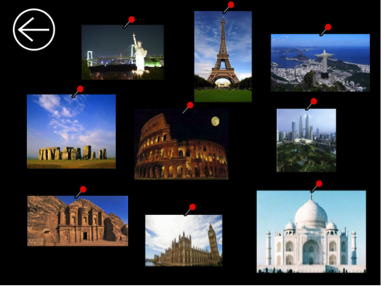
\includegraphics{Jumper}

\begin{enumerate}
\item After Clicking the Jumper Icon among the main page, users see above the image which shows photographs of tourist attraction they want to go.   
\item By using gyroscope and magenetic button, users will find the attraction place which they want to go and will choose the photograph.\\
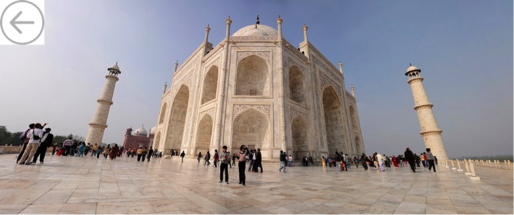
\includegraphics{View}
\item Users are able to trip the attraction zone as if they are in there. Because we want 360? aerial panorama view, we solve this problem using Google maps street view API. If the tour is over, users could exit by using back button.
\end{enumerate}

%subsubsection 6
\subsubsection{Specification of Cine}
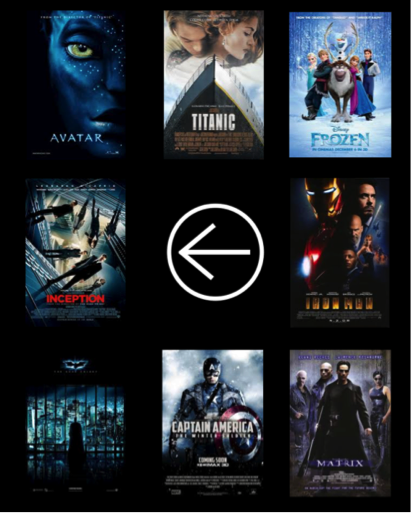
\includegraphics{Cine}

\begin{enumerate}
\item After Clicking the Cine Icon among the main page, users see above the image which shows movie posters you download in smartphone.   
\item Like main page, by using gyroscope and magenetic button, users will find the movie which they want to see and will choose the movie
\item Users could watch the movie as if they feel in movie cinema.Users can pause movie by magnetic buttom and exit from cinema by back buttom located left-top in display.
\end{enumerate}

*testing testing by seungkyu




\end{document}
